\subsection{Symbolic Representation}

Representing the uncertain components of a query's output symbolically as a c-table makes a wide variety of integration techniques available for use in evaluating the statistical characteristics of the expression.  If our risk-management application assumes a general model of customer profit and customer satisfaction that relies on queries to create correlations between them, the sampler can detect this lack of dependency, estimate profit and probability of dissatisfaction separately, and combine the two afterwards.  Even with relatively straightforward integration techniques, additional knowledge of this form has a profoundly positive impact on the efficiency and accuracy with which expectations of query results can be computed.

Accuracy is especially relevant in cases where the integral has no closed form and exact methods are unavailable.  This is the case in a surprising range of practical applications, even when strong simplifying assumptions are made about the input data.  For example, even if the input data contains only independent variables sampled from well-studied distributions (e.g., the normal distribution), it is still possible for queries to create complex statistical dependencies in their own right.  It is well known, at least in the case of discrete and finite probability distributions, that relational algebra on block-independent-disjoint tables can construct any finite probability distribution\ \cite{1325861,IL1984}.

PIP represents probabilistic data values symbolically via random variables defined in terms of parametrized probability distribution classes.  PIP supports several generic classes of probability distributions (e.g., Normal, Uniform, Exponential, Poisson), and may be extended with additional classes.  Variables are treated as opaque while they are manipulated by traditional relational operators.  The result is a symbolic representation of uncertainty, a c-table \cite{IL1984,GT2006, KochMayBMS2008}.  As the final stage of the query, special operators defined within PIP compute expectations and moments of the uncertain data, or sample the data to generate histograms.  

These expectation operators are invoked with an unbiased, lossless representation of the expression to be evaluated.  Because the variables have been treated as opaque, the expectation operator can obtain information about the distribution a variable corresponds to.  Developers can (but need not) provide supplemental information (e.g., functions defining the PDF and the CDF) about distributions they extend PIP with.  The operator can exploit this additional information to accelerate the sampling process, or potentially even sidestep it entirely.  For example, if a query asks for the probability that a variable will fall within specified bounds, the expectation operator can compute it with at most two evaluations of the variable's CDF.

Because the symbolic representation PIP uses is lossless, intermediate query results or views may be materialized.  Expectations of values in these views or subsequent queries based on them will not be biased by estimation errors introduced by materializing the view.  This is especially useful when a significant fraction of query processing time is devoted to managing deterministic data (eg, to obtain parameters for the model's variables).  Not only can this accelerate processing of commonly used subqueries, but it makes online sampling feasible; the sampler need not evaluate the entire query from scratch to generate additional samples.



%%%%%%%%%%%%%%%%


\begin{example}\em
Now consider using c-tables. The result of the relational algebra part of the
above query can be easily computed as
\[
\begin{tabular}{c|c|c}
R & Price & Condition \\
\hline
& $X_1$ & $X_2 \ge 7$ \\
\end{tabular}
\]
without looking at $p$.
This c-table compactly represents all data still relevant after the
application of the relational algebra part of the query, other than $p$,
which remains unchanged.
Sampling from R to compute
\begin{verbatim}
select expected_sum(Price) from R;
\end{verbatim}
is a much more focused effort.
First, we only have to consider the random variables relating to Joe;
but determining that random variable $X_2$ is relevant while $X_4$
is not requires
executing a query involving a join. We want to do this query first, before
we start sampling.

Second, assume that delivery times are
independent from sales volumes. Then we can approximate the
query result
by first sampling an $X_2$ value and only sampling an $X_1$ value if $X_2 \ge 7$.
Otherwise, we use $0$ as the $X_1$ value.
If $X_2 \ge 7$ is relatively rare (e.g., the average shipping times to NY are
very slow, with a low variance), this may reduce the amount of samples
for $X_1$ that are first computed and then discarded without seeing use
considerably.
If CDFs are available, we can of course do even better.
%
\end{example}



%%%%%%%%%%%%%%%%%%%%%%%%%%%%%



%

\begin{figure}[!]
\begin{center}
\begin{tabular}{rc}
& Query
\\
%\\
%\hline
\\
\begin{tabular}{r}
query \\
evaluation
\end{tabular}
&
\framebox{
\begin{tabular}{c}
\framebox{
\begin{tabular}{p{4.2cm}}
computing probabilities, \\
moments, and statistical tests
\end{tabular}
}
\\[3ex]
\framebox{
\begin{tabular}{p{4.2cm}}
query plans on c-tables
\end{tabular}
}
\end{tabular}
}
\\[7ex]
\begin{tabular}{l}
data \\
store
\end{tabular}
&
\framebox{
\begin{tabular}{c}
\framebox{
\begin{tabular}{p{4.2cm}}
(probabilistic) c-tables
\end{tabular}
}
\\[2ex]
\framebox{
\begin{tabular}{p{4.2cm}}
succinct representation of \\
joint distribution of random \\
variables (exchangeable)
\end{tabular}
}
\end{tabular}
}
\end{tabular}
\end{center}
\caption{Pip Query Engine Architecture.}
\label{fig:arch}
\end{figure}



\begin{figure}
\begin{center}
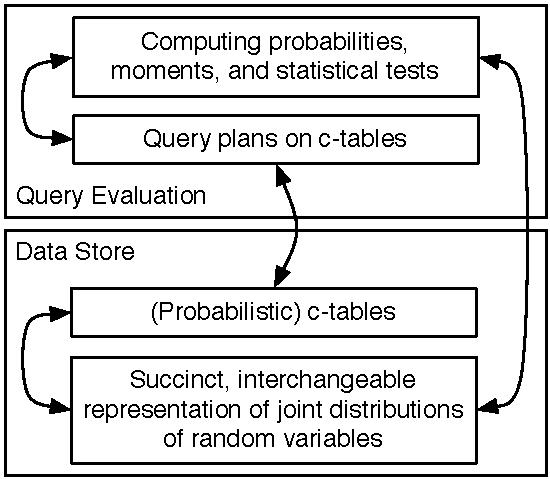
\includegraphics[width=2in]{graphics/arch.pdf}
\vspace*{-0.1in}
\caption{Pip Query Engine Architecture}
\label{fig:arch}
\end{center}
\vspace*{-0.35in}
\end{figure}
The goal of PIP is to evaluate queries on variables sampled from both discrete and continuous distributions as well as to provide tools to aid in the statistical analysis of those results.  Uncertainty in PIP is represented via random variables.  When instantiating a random variable, users specify both a distribution for the variable to be sampled from, and a parameter set for that distribution.  A single variable may appear simultaneously at multiple points within the database, so PIP assigns each variable a unique identifier that allows sampling processes to generate consistent values for the variable.

In addition to representing uncertainty in values for individual cells in a table, PIP represents per-tuple uncertainty with c-tables.  Each tuple is tagged with a condition that must hold for the variable to be present in the table.  C-table conditions are expressed as a boolean equation of \textit{atoms}, arbitrary inequalities of random variables.  The independent probability, or \textit{confidence} of the tuple is the probability of the condition being satisfied.  

\subsection{Random Variables}
Every random variable is created from by specifying a distribution and a set of parameters for that distribution.  For example, we write $[X=>Normal(\mu,\sigma^2)]$ to represent a random variable named X that follows a Normal distribution with a mean of $\mu$ and a standard deviation of $\sigma^2$.  In this way, PIP is agnostic to the distribution which a variable is sampled from; arbitrary problem-specific distributions may be created and seamlessly integrated into PIP's infrastructure.  

When defining a distribution, programmers need only include a mechanism for sampling from that distribution.  However, if it is possible to efficiently compute or estimate the distribution's probability density function ($PDF$), cumulative distribution function ($CDF$), or inverse cumulative distribution function ($CDF^{-1}$), these may be included to increase PIP's efficiency.  The process of defining a variable distribution is described further in Section \ref{sec:implementation}.  

Though PIP abstracts the details of a variable's distribution from query evaluation, it distinguishes between discrete and continuous distributions.  As described in Section \ref{sec:background}, existing research into c-tables has demonstrated efficient ways of querying variables sampled from discrete distributions.  PIP employs similar techniques when it is possible to do so.

Multiple continuous random variables may be combined algebraically into a random variable expression.  Random variable expressions may be used to define joint distributions, to build more complex distributions, or may be created as a side effect of query evaluation.  Though random variable expressions are interchangeable with regular random variables in general, there are several instances where they receive special treatment.  In particular, it is necessary to ensure that within a given sample all instances of a given random variable assume the same value; the expectation of a random variable expression is obtained based on a consistent set of samples for all of its component random variables.

Finally, constraint predicates, or atoms are conditional formulas of random variables.  Such formulas may be equalities if all variables in the fomula are discrete, otherwise they must be an inequality; the probability of a continuous variable adopting an exact value is zero.  Given a constraint atom $C$, its probability $P[C]$ is the probability of selecting variable assignments that satisfy the formula.  Constraint atoms are used to express a tuple's condition.  By adding constraint atom columns to a table, a tuple's presence in the table becomes dependent on the constraint atom being true; the tuple's presence is based on the conjunction of all its component atoms.

\subsection{Variable Definition}
Before evaluating a query on random variables, the variables must first be defined.  This process takes one of two forms.  PIP uses a repair-key operator similar to that used in \cite{KochMayBMS2008} to define discrete distributions.  Conceptually, this operator identifies tuples that share key values, and ensures that only one of the two tuples is present in the database at any given moment.  

Continuous variables may be created inline with the create-variable operation.  This function takes a distribution class and parameters, and outputs a new variable.  For example, the following query outputs a variable delivery time for a given order.

\begin{verbatim}
select orders.order_id, orders.item_id,
       CREATE_VARIABLE (`Normal', params.mean,
         params.std_dev) AS delivery_time
from   orders, params
where  orders.item_id = params.item_id;
\end{verbatim}

\subsection{Query Processing}
Query evaluation proceeds in two phases: Query and Sampling.  During the query phase, PIP evaluates a query rewritten to employ the c-tables relational algebra extensions described in Section \ref{sec:background}.  Selection clauses not involving random variables are handled traditionally, while those involving one or more random variables instead tag the output tuple with an equivalent condition clause.  For example, the query:

\begin{verbatim}
select *
from   input_table
where  fixed_column = 3 and 4 > variable_column;
\end{verbatim}
%
is rewritten to
%
\begin{verbatim}
select *, define_constraint(4, variable_column)
from   input_table
where  fixed_column = 3;
\end{verbatim}

Queries are also modified to ensure that these newly created constraint columns interact with projections properly.  All select statements are modified to automatically output all constraint columns in their input tables and subqueries.  The only exception to this rule is in the case of sampling selection.  Behaving similarly to aggregate selects, a sampling select projects away uncertainty by including a sampling operator such as expectation(), or conf().  Note that aggregate and sampling selects are not mutually exclusive.  Indeed, due to the complexity of losslessly representing arbitrary aggregate output conditions (An aggregate can generate $2^{N}$ distinct outputs in the number of input rows, though these can be encoded in linear space), PIP requires that aggregate selects perform sampling. 

\subsection{Per-Row Sampling}
Given a target expression (that may contain random values) as well as a set of constraints, the sampler computes the expression's expectation by first subdividing the problem as described in Section \ref{subsec:independence}.  These groups are subsequently divided into two categories: Groups containing at least one variable contained in the target expression are marked for sampling.  The volume of the probability space defined by all constraints must be computed, but storage overheads may be avoided for those groups not directly relevant to the target expression; these groups are marked for integration.  Additionally, if such a group contains only one variable, the integral may be computed exactly using a single call to the variable's CDF if one is available.

The remaining groups are sampled to obtain values for Monte-Carlo estimation of the target expression's expectation.  By default, these samples are obtained through naive rejection sampling.  Variables are selected from the distribution $\frac{\chi(\vec{x})p(\vec{x})}{\int_{\vec{a}} \chi(\vec{a})p(\vec{a})}$ by sampling according to $p(\vec{x})$ and discarding values that do not satisfy $\phi(\vec{x})$.  Finally, the expectation value computed is re-normalized according to the frequency with which samples are discarded.

If any of the variables have a CDF available, PIP first attempts to obtain weak bounds on the variable as described in Section \ref{subsec:icdf}.  If such bounds are available, PIP can use the variable's CDF and inverse CDF to restrict sampling to within the weak bounds.  If the weak bounds are actually tight bounds, no samples will be discarded.  However, even if some samples are rejected, the bounds reduce the drop frequency.  When computing the volume of the probability space defined by the constraints, the values are re-normalized according to the fraction of the CDF located within the bounds.

A final option available to PIP is the Metropolis algorithm.  Metropolis has a high initialization cost: Prior to sampling, at least one value $\vec x$ satisfying $\theta(\vec x)$ must be found (though it need not be selected according to any specific probability distribution), and a significant number of burn-in iterations must be run and discarded.  Furthermore, every sampling step requires many Metropolis iterations to achieve sufficiently independent samples.  However, Metropolis is guaranteed to stay within the constraint bounds and no samples will be rejected.  Thus, we can estimate the work required for both Metropolis and Naive rejection sampling.

$$W_{metropolis} = C_{burn\ in} + [\#\ samples] \cdot C_{steps\ per\ sample}$$
$$W_{naive} = \frac{1}{1-P[reject]} \cdot [\#\ samples]$$

By generating a small number of samples for the subgroup, PIP generates a rough estimate of $P[reject]$.  If this value is lower than $\frac{1}{\frac{C_{burn\ in}}{[\#\ samples]} + C_{steps\ per\ sample}}$, Metropolis sampling is used instead of rejection sampling.  Note that if CDFs are available for one or more component variables, PIP uses the probability of rejecting samples chosen from within the available weak bounds.

The single-row sampling process is sumarized in Figure \ref{fig:roadmap}

\begin{figure}
\begin{center}
%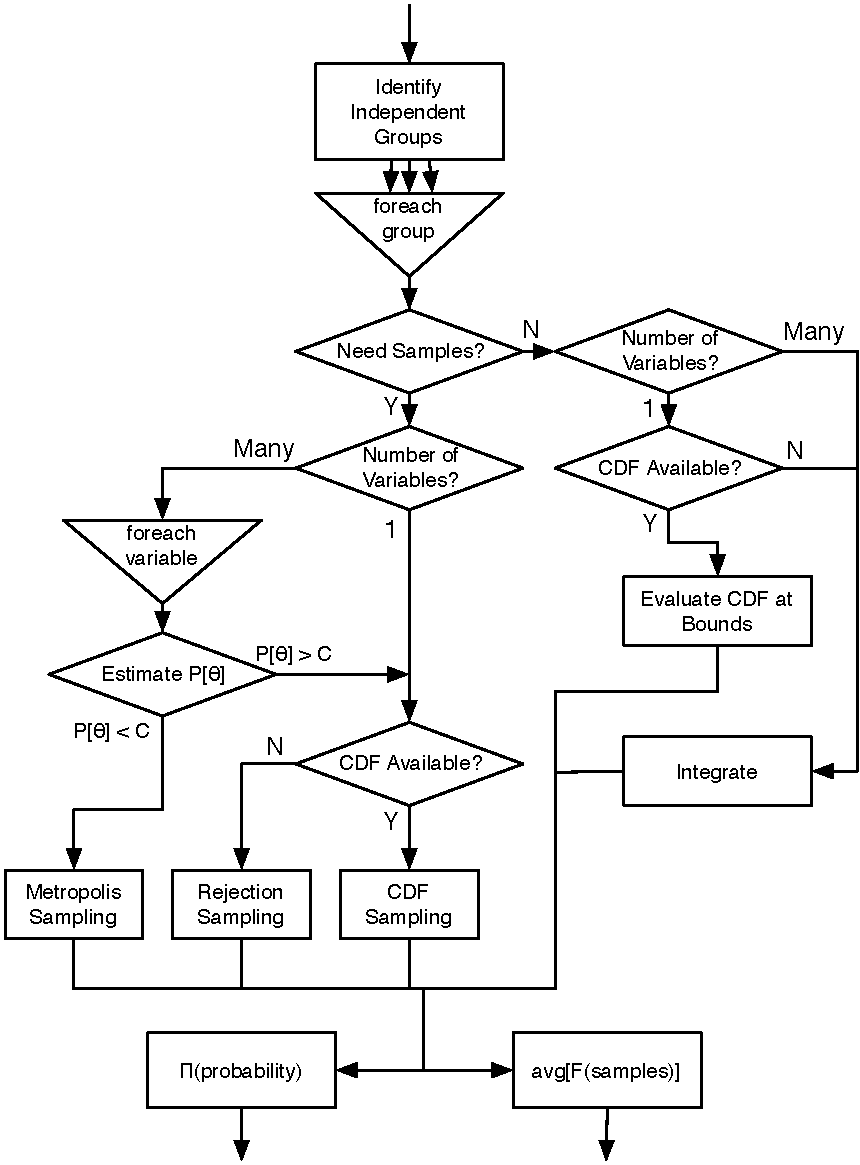
\includegraphics[width=3in]{graphics/roadmap.pdf}
\begin{enumerate}
\item 
\end{enumerate}
\caption{\textbf{The PIP Single-Row sampling process}}
\vspace*{-0.2in}
\label{fig:roadmap}
\end{center}
\vspace*{-0.15in}
\end{figure}

\subsection{Aggregate Sampling}
The complexity introduced by aggregate operations, coupled with the frequency with which they appear at the root of a query plan, makes them an ideal point at which to perform sampling.  We begin with the simplest form of aggregate expectation, that of an aggregate that obeys linearity of expectation ($\left<f(\vec{x})\right> = f(\vec{\left<x\right>})$), such as sum().  

Such aggregates are straightforward to implement: per-row expectations of $f(\vec x)\chi(\vec x)$ are computed, and aggregated (e.g., summed up).  Of note however, is the effect that the operator has on the variance of the result.  In the case of sum(), each expectation can be viewed as a Normally distributed random variable with a shared, predetermined variance.  By the law of large numbers, the sum of a set of $N$ random variables with equal variance $\sigma$ has a variance of $\frac{\sigma}{\sqrt{N}}$.  In other words, when computing the expected sum of $N$ variables, we can reduce the number of samples taken for each individual element by a factor of $\frac{1}{\sqrt{N}}$.

If the operator does not obey linearity of expectation (e.g., computing the maximum), either the aggregate must be designed with expectation computation in mind, or the aggregate must be run on a set of sampled worlds in parallel.  This latter technique is a worst-case approach to the problem; it may be necessary to re-run the aggregate if an insufficient number of sample worlds are generated. Note however, that this is still more efficient than re-running the entire query.

The max() aggregate can be implemented more efficiently, particularly when the target expression is a constant (ie, a value that is certain for the row in question).  Given a table table sorted over descending values of the target expression, PIP estimates the probability that the first element in the table (the highest value) is present.  The aggregate expectation is initialized as the product of this probability and the first element.  The second term is maximal only if the first term is not present; when computing the probability of the second term, we must compute the probability of all the second term's constraint atoms being fulfilled while at least one of the first atom's terms is not fulfilled.  Though the complexity of this process is exponential in the number of rows, the probability of each successive row being maximal drops exponentially.  




%%%%%%%%%%%%%%%%%%%%%%%%%%%%%



Note that  a tuple can be removed  from a c-table if  its condition is
inconsistent.   Conditions  can   become  inconsistent   by  combining
contradictory conditions  using conjunction,  which may happen  in the
implementations of the operators selection, product, and difference.

A condition is consistent if there is a variable assignment that makes
the condition true. For general boolean formulas, deciding consistency
is computationally  hard. But we do  not need to decide  it during the
evaluation of relational  algebra operations.  Rather, we exploit straightforward cases of inconsistency to clean-up c-tables and reduce their sizes.
We rely on the later 
Monte Carlo simulation phase to enforce the remaining inconsistencies.
%
\begin{enumerate}
\item The consistency of conditions not involving variable values is always immediately apparent.
\item Conditions $X_i = c_1 \land X_i = c_2$ with constants $c_1 \neq c_2$ are always inconsistent.
\item Equality conditions over continuous variables $Y_j = (\cdot)$, with the exception of the identity $Y_j = Y_j$, are not inconsistent but can be treated as such (the probability mass will always be zero).  Similarly, conditions $Y_j \neq (\cdot)$, with the exception of $Y_j \neq Y_j$, can be treated as true and removed.
\item Other forms of inconsistency can also be detected where it is efficient to do so.
\end{enumerate}

With  respect to  discrete variables,  inconsistency detection  may be
further simplified.  Rather than using abstract representations, every
row containing  discrete variables  may be exploded  into one  row for
every possible valuation.  Condition atoms matching each variable to its
valuation  are used  to ensure  mutual exclusion  of each  row.  Thus,
discrete variable columns may be  treated as constants for the purpose
of  consistency checks.  As  shown in  \cite{AJKO2008}, deterministic
database  query optimizers  do  a satisfactory  job  of ensuring  that
constraints over discrete variables are filtered as soon as possible.

Given  tables  in which  all  conditions  are  conjunctions of  atomic
conditions and  the query does not employ  duplicate elimination, then
all conditions  in the output  table are conjunctions.  Thus  it makes
sense to particularly optimise this scenario \cite{AJKO2008}.
In the case of positive
relational algebra  with the duplicate elimination  operator (i.e., we
trade  duplicate   elimination  against  difference),   we  can  still
efficiently  maintain  the  conditions  in  DNF,  i.e.,  as  a  simple
disjunction of conjunctions of atomic conditions.

Without loss of generality, the model can be limited to conditions that
are conjunctions of
constraint  atoms.  Generality  is maintained by  using bag  semantics to
encode disjunctions. This  restriction   provides   several  benefits.
First,
constraint  validation is  simplified;  A pairwise  comparison of  all
atoms in the clause is  sufficient to catch the inconsistencies listed
above.   As an additional  benefit, if  all atoms  of a  clause define
convex and  contiguous regions in the space $\vec{x},\vec{y}$, these same
properties are also shared by their intersection.
%This benefits  sample generation in ways that will be discussed later.




\subsection{Probabilistic c-tables; expectations}
\label{sec:montecarlo}


A \textit{probabilistic  c-table} (cf.\ \cite{GT2006, KochMayBMS2008}) is a c-table in  which each variable is
simply considered a (discrete  or continuous) {\em random variable}\/,
and a joint probability distribution is given for the random variable.
As  a convention,  we will  denote  the discrete  random variables  by
$\vec{X}$ and the continuous ones by $\vec{Y}$.  Throughout the paper,
we  will  always  assume  without  saying that  {\em  discrete  random
variables have a finite domain}\/.

We    will   assume    a    suitable   function    $p(\vec{X}=\vec{x},
\vec{Y}=\vec{y})$ specifying a joint distribution which is essentially
a  PDF  on the  continuous  and a  probability  mass  function on  the
discrete variables.  To clarify  this, $p$ is such that
we can define the expectation of a function $q$ as
\[
E[q] =
\sum_{\vec{x}} \int_{y_1} \cdots \int_{y_n}
p(\vec{x}, \vec{y}) \cdot q(\vec{x}, \vec{y}) \; d \vec{y}
\]
and approximate it as
\[
\frac{1}{n} \cdot \sum_{i=1}^n q(\vec{x}_i, \vec{y}_i)
\]
given samples $(\vec{x}_1, \vec{y}_1), \dots, (\vec{x}_n, \vec{y}_n)$ from
the distribution $p$.

%ck: That's BS, moments are covered by expectations.
%Throughout this paper, we will consider expectations and their special
%cases (such as event probabilities), but we will not discuss higher moments.
%Note though that the extension of our framework is conceptually simple.


We can specify events (sets of possible worlds) via Boolean conditions
$\phi$  that  are true  on  a  possible  world (given  by  assignment)
$\theta$  iff the condition  obtained by  replacing each  variable $x$
occurring  in  $\phi$  by  $\theta(x)$ is  true.   The  characteristic
function  $\chi_\phi$  of condition  (event)  $\phi$  returns  1 on  a
variable  assignment  if  it   makes  $\phi$  true  and  returns  zero
otherwise.   The probability  $\Pr[\phi]$  of event  $\phi$ is  simply
$E[\chi_\phi]$.

The expected  sum of a function $h$  applied to the tuples  of a table
$R$,
\begin{verbatim}
select expected_sum(h(*)) from R;
\end{verbatim}
can be computed as
\[
E \Big[ \sum_{\vec{t}  \in R}  h(\vec{t}) \Big]  =
E \Big[ \sum_{(t, \phi) \in C_R} \chi_\phi \cdot h(t) \Big] =
\sum_{(t, \phi) \in C_R} E \Big[ \chi_\phi \cdot (h \circ t) \Big]
\]
(the latter by linearity of expectation).
%, or equivalently
%\[
%   \sum_{(t,  \phi) \in  C_R} \sum_{\vec{x}}  \cdot  \int_{y_1} \cdots
%   \int_{y_n}  p(\vec{x}, \vec{y})  \cdot  \chi_\phi(\vec{x}, \vec{y})
%   \cdot h(t[\vec{x}, \vec{y}]) \; d \vec{y}.
%\]
Here $t(\vec{x}, \vec{y})$ denotes
the tuple $t$, where any variable that may occur is replaced by
the value assigned to it in $(\vec{x}, \vec{y})$.


\begin{example}\em
Returning to our running example, for $C_R = \bagopen (x_1, x_2 \ge 7) \bagclose$, the expected sum of prices is
\begin{multline*}
   \sum_{(t,  \phi) \in  C_R} \cdot  
   \int_{x_1} \cdots
   \int_{x_4}  p(\vec{x})  \cdot  \chi_\phi(\vec{x})
   \cdot t(\vec{x}).\mathrm{Price} \; d \vec{y}
= \\
   \int_{x_1} \cdots
   \int_{x_4}  p(\vec{x})  \cdot  \chi_{X_2 \ge 7}(\vec{x})
   \cdot x_1 \; d \vec{y}.
\end{multline*}
\punto
\end{example}


{\bf Counting and group-by}\/.
Expected count aggregates are obviously special cases of expected sum
aggregates where $h$ is a constant function $1$.
We generally consider expected sum aggregates with grouping by (continuously)
uncertain columns to be of doubtful value.
Group-by on nonprobabilistic columns (i.e., which contain no random variables)
poses no difficulty in the c-tables framework: the above summation simply
proceeds within groups of tuples from $C_R$ that agree on the group columns.
In particular, by delaying any sampling process until after the relational
algebra part of the query has been evaluated on the c-table representation,
we find it easy to create as many samples as we need for each group in a 
goal-directed fashion. This is a considerable strong point of the c-tables
approach used in PIP.


